\documentclass[11pt]{article}

\usepackage[margin=1in]{geometry}
\usepackage[T1]{fontenc}
\usepackage{lmodern}
\usepackage{microtype}
\usepackage{amsmath,amssymb,amsthm,mathtools}
\usepackage[dvipsnames]{xcolor}
\usepackage[most]{tcolorbox}
\usepackage{tikz}
\usetikzlibrary{decorations.markings}
\usepackage{enumitem}
\usepackage{tocloft}
\usepackage[hidelinks]{hyperref}

\definecolor{courseblue}{HTML}{1F4E79}
\definecolor{lightblue}{HTML}{EAF2F8}
\definecolor{lightgreen}{HTML}{EAF7EA}
\definecolor{lightpink}{HTML}{FCE8EF}
\definecolor{lightyellow}{HTML}{FFF8D6}
\definecolor{warningyellow}{HTML}{D6A000}
\definecolor{exercisebg}{HTML}{D6E6F5}
\definecolor{exerciseframe}{HTML}{1F4E79}
\definecolor{examplebg}{HTML}{F4FAFE}
\definecolor{exampleframe}{HTML}{85C1E9}
\definecolor{darkgray}{HTML}{333333}
\definecolor{lightorange}{HTML}{FDEBD8}
\definecolor{orangeframe}{HTML}{E08A3C}

\setlength{\parindent}{0pt}
\setlength{\parskip}{0.65em}
\setlist[itemize]{topsep=0.25em,itemsep=0.15em}
\renewcommand{\cftsecleader}{\cftdotfill{\cftdotsep}}
\renewcommand{\cftsubsecleader}{\cftdotfill{\cftdotsep}}

\theoremstyle{plain}
\newtheorem{theorem}{Theorem}[section]
\newtheorem{proposition}[theorem]{Proposition}
\newtheorem{lemma}[theorem]{Lemma}
\newtheorem{corollary}[theorem]{Corollary}
\theoremstyle{definition}
\newtheorem{definition}[theorem]{Definition}
\newtheorem{example}[theorem]{Example}
\newtheorem{exercise}[theorem]{Exercise}
\theoremstyle{remark}
\newtheorem*{remark}{Remark}
\newtheorem*{fact}{Fact}
\newtheorem*{warning}{Warning}

\tcolorboxenvironment{definition}{
  enhanced,
  unbreakable,
  colback=lightgreen,
  colframe=ForestGreen,
  boxrule=0.7pt,
  arc=2pt,
  left=6pt,
  right=6pt,
  top=5pt,
  bottom=5pt
}

\tcolorboxenvironment{warning}{
  enhanced,
  colback=lightyellow,
  colframe=warningyellow,
  boxrule=0.7pt,
  arc=2pt,
  left=6pt,
  right=6pt,
  top=5pt,
  bottom=5pt
}

\tcolorboxenvironment{exercise}{
  enhanced,
  colback=exercisebg,
  colframe=exerciseframe,
  boxrule=1pt,
  arc=2pt,
  left=6pt,
  right=6pt,
  top=5pt,
  bottom=5pt
}

\tcolorboxenvironment{example}{
  enhanced,
  colback=examplebg,
  colframe=exampleframe,
  boxrule=0.7pt,
  arc=2pt,
  left=6pt,
  right=6pt,
  top=5pt,
  bottom=5pt
}

\numberwithin{equation}{section}

\newcommand{\be}{\begin{eqnarray}}
\newcommand{\ee}{\end{eqnarray}}
\newcommand{\C}{\mathbb{C}}
\newcommand{\R}{\mathbb{R}}
\newcommand{\N}{\mathbb{N}}

\DeclareMathOperator{\Hol}{\mathcal{H}\mathrm{ol}}
\DeclareMathOperator{\Real}{Re}
\DeclareMathOperator{\Imag}{Im}
\newcommand{\A}{\mathcal{A}}
\newcommand{\CT}{\C[[T]]}
\newcommand{\CLT}{\C((T))}
\tcbset{breakable}
\begin{document}

\begin{center}
  \colorbox{lightblue}{%
    \begin{minipage}{0.94\textwidth}
      \vspace{0.55em}
      \begin{tabular*}{\textwidth}{@{\extracolsep{\fill}}lr}
        {\color{courseblue}\bfseries\LARGE Lecture 14} &
        {\color{courseblue}\bfseries\LARGE MATH 411}\\[0.35em]
        \textbf{Fall 2026} & \textbf{Date: Oct 7, 2026}\\
        & \textbf{Instructor: Manish Patnaik}
      \end{tabular*}
      \vspace{0.45em}
    \end{minipage}}
\end{center}

\setcounter{tocdepth}{1}
\tableofcontents
\vspace{0.45em}

% Sources: handwritten Lecture 14 (all six pages) and Lecture 15 (pages 1--4).
% Stop before "Contour integrals of holomorphic functions on continuous curves".
\section{Review of Lecture 13: primitives and Cauchy's theorem}
Throughout this lecture, a \emph{path} means a continuous, piecewise
continuously differentiable curve.

\textbf{Primitives and endpoint evaluation.} A primitive of a continuous
function $f$ on an open set $U$ is a holomorphic function $g$ on $U$ with
$g'=f$. If $\gamma\colon[a,b]\to U$ is a path, the chain rule gives
\begin{equation}\label{eq:review-primitive}
 \int_\gamma f(z)\,dz=g\bigl(\gamma(b)\bigr)-g\bigl(\gamma(a)\bigr).
\end{equation}
Thus the integral depends only on the endpoints, and it is zero when
$\gamma$ is closed. Conversely, on an open connected set, if every closed
path integral of a continuous $f$ vanishes, then
$g(z)=\int_{z_0}^z f(w)\,dw$ is well-defined and is a primitive of $f$.

\textbf{Primitives on a disc.} In Lecture~13 we showed that if $f$ is
continuous on a disc $D$ and $\int_{\partial R}f=0$ for every 
rectangle $R\subseteq D$, then $f$ has a primitive on $D$. We constructed
it by integrating from the centre along a horizontal and a vertical
segment. The rectangle condition makes the two orders agree, and the
ML\footnote{This is the estimate $|\int_{\gamma} f| \leq \max_{z \in \gamma} |f(z)| \, L_{\gamma}$ where $L_{\gamma}$ is the arclength of $\gamma$. The "M" stands for max, and "L" for arclength } estimate gives $g'=f$.

\begin{theorem}[Cauchy's theorem on a disc]\label{thm:review-cauchy}
Let $D\subseteq\C$ be an open disc and let $f$ be holomorphic on $D$.
Then $f$ has a primitive on $D$, and for every closed path $\gamma$ in $D$,
\begin{equation}\label{eq:review-cauchy}
 \boxed{\displaystyle\int_\gamma f(z)\,dz=0.}
\end{equation}
\end{theorem}
\begin{proof}
Goursat's theorem gives $\int_{\partial R}f=0$ for every rectangle
$R\subseteq D$. The primitive construction above applies, and
\eqref{eq:review-primitive} gives zero because the endpoints agree.
\end{proof}

In particular, if $f$ is \emph{entire}, its integral over every closed
path is zero: the compact image of the path lies in some disc.
The domain matters: $1/z$ is holomorphic on $\C\setminus\{0\}$, but
its integral around the counterclockwise unit circle is $2\pi i$.
Local primitives need not give a primitive on the whole domain.

Today we combine Cauchy's theorem with the ML estimate to compute real
integrals by choosing suitable closed contours.

\newpage
\section{The Gaussian integral and its Fourier transform}
% Handwritten Lecture 14, page 1.
\subsection{The Gaussian integral}
First recall the real-variable calculation
\begin{equation}\label{eq:gaussian}
 \int_{-\infty}^{\infty}e^{-\pi x^2}\,dx=1.
\end{equation}
Let $I$ denote this integral. It converges: for $|x|\geq1$,
$e^{-\pi x^2}\leq e^{-\pi|x|}$. Since the integrand is nonnegative, we may
write the product as a double integral and use polar coordinates:
\begin{align*}
 I^2
 &=\int_{\R^2}e^{-\pi(x^2+y^2)}\,dx\,dy\\
 &=\int_0^{2\pi}\int_0^\infty e^{-\pi r^2}r\,dr\,d\theta
 =2\pi\left[-\frac{e^{-\pi r^2}}{2\pi}\right]_{0}^{\infty}=1.
\end{align*}
As $I>0$, we obtain $I=1$.

\subsection{A family of oscillatory integrals}
For a fixed $\xi\in\R$, consider
\[
 F(\xi)=\int_{-\infty}^{\infty}e^{-\pi x^2}e^{-2\pi i x\xi}\,dx.
\]
This integral converges absolutely, since $|e^{-2\pi i x\xi}|=1$.
When $\xi=0$, it is \eqref{eq:gaussian}. The general answer is again a
Gaussian.
\begin{theorem}\label{thm:fourier-gaussian}
For every $\xi\in\R$,
\begin{equation}\label{eq:fourier-gaussian}
 \boxed{\displaystyle
 \int_{-\infty}^{\infty}e^{-\pi x^2}e^{-2\pi i x\xi}\,dx
 =e^{-\pi\xi^2}.}
\end{equation}
\end{theorem}


% Handwritten Lecture 14, pages 2--4.
\subsection{Shifting the contour}
\begin{proof}[Proof of Theorem~\ref{thm:fourier-gaussian}]
The substitution $x\mapsto-x$ gives $F(-\xi)=F(\xi)$, so it is enough to
consider $\xi>0$; the case $\xi=0$ is already known.

Let $f(z)=e^{-\pi z^2}$, which is entire. For $R>0$, take the rectangular
contour with vertices $-R$, $R$, $R+i\xi$, and $-R+i\xi$, oriented
counterclockwise.
\begin{center}
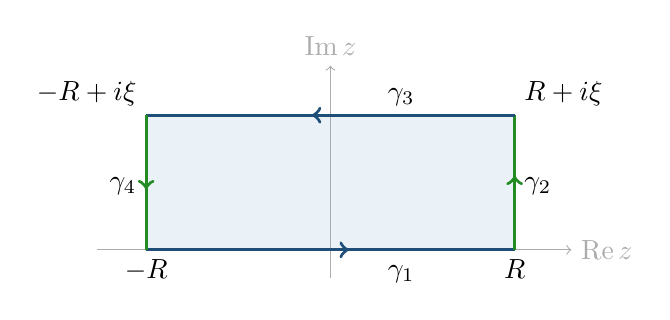
\begin{tikzpicture}[scale=0.9,
 decoration={markings,mark=at position 0.55 with {\arrow{>}}}]
 \fill[lightblue] (-2.6,0) rectangle (2.6,1.9);
 \draw[gray!65,->] (-3.3,0)--(3.4,0) node[right]{$\Real z$};
 \draw[gray!65,->] (0,-0.4)--(0,2.6) node[above]{$\Imag z$};
 \draw[very thick,courseblue,postaction={decorate}] (-2.6,0)--(2.6,0);
 \draw[very thick,ForestGreen,postaction={decorate}] (2.6,0)--(2.6,1.9);
 \draw[very thick,courseblue,postaction={decorate}] (2.6,1.9)--(-2.6,1.9);
 \draw[very thick,ForestGreen,postaction={decorate}] (-2.6,1.9)--(-2.6,0);
 \node[below] at (-2.6,0){$-R$}; \node[below] at (2.6,0){$R$};
 \node[above left] at (-2.6,1.9){$-R+i\xi$};
 \node[above right] at (2.6,1.9){$R+i\xi$};
 \node[below] at (1,-0.08){$\gamma_1$};
 \node[right] at (2.6,0.9){$\gamma_2$};
 \node[above] at (1,1.9){$\gamma_3$};
 \node[left] at (-2.6,0.9){$\gamma_4$};
\end{tikzpicture}
\end{center}
Cauchy's theorem gives
\begin{equation}\label{eq:rectangle}
 \int_{\gamma_1}f+\int_{\gamma_2}f+
 \int_{\gamma_3}f+\int_{\gamma_4}f=0.
\end{equation}
We may parametrize the four sides by
\[
\begin{array}{lll}
 \gamma_1(t)=t, & -R\leq t\leq R, & \gamma_1'(t)=1,\\[2pt]
 \gamma_2(t)=R+it, & 0\leq t\leq\xi, & \gamma_2'(t)=i,\\[2pt]
 \gamma_3(t)=-t+i\xi, & -R\leq t\leq R, & \gamma_3'(t)=-1,\\[2pt]
 \gamma_4(t)=-R+i(\xi-t), & 0\leq t\leq\xi, & \gamma_4'(t)=-i.
\end{array}
\]
\textbf{The bottom side.} By \eqref{eq:gaussian},
\[
 \int_{\gamma_1}f=\int_{-R}^{R}e^{-\pi t^2}\,dt\longrightarrow1
 \qquad(R\to\infty).
\]
\textbf{The vertical sides.} On $z=R+it$,
\[
 (R+it)^2=R^2+2iRt-t^2,
 \qquad |e^{-\pi(R+it)^2}|=e^{-\pi R^2}e^{\pi t^2}.
\]
Hence
\[
 \left|\int_{\gamma_2}f\right|
 \leq e^{-\pi R^2}\int_0^\xi e^{\pi t^2}\,dt
 \leq \xi e^{\pi\xi^2}e^{-\pi R^2}\longrightarrow0.
\]
Exactly the same estimate holds on the left side $\gamma_4$.


% Handwritten Lecture 14, pages 4--5.
\textbf{The top side.} Its orientation is from right to left. Using the
parametrization above,
\begin{align*}
 \int_{\gamma_3}f
 &=-\int_{-R}^{R}e^{-\pi(-t+i\xi)^2}\,dt\\
 &=-e^{\pi\xi^2}\int_{-R}^{R}e^{-\pi t^2}e^{2\pi it\xi}\,dt\\
 &=-e^{\pi\xi^2}\int_{-R}^{R}e^{-\pi x^2}e^{-2\pi ix\xi}\,dx,
\end{align*}
where the last equality uses $x=-t$. Absolute convergence gives
\[
 \int_{\gamma_3}f\longrightarrow-e^{\pi\xi^2}F(\xi).
\]
Taking $R\to\infty$ in \eqref{eq:rectangle}, we obtain
\[
 1+0-e^{\pi\xi^2}F(\xi)+0=0.
\]
Therefore $F(\xi)=e^{-\pi\xi^2}$, as claimed.
\end{proof}

\begin{corollary}[Real and imaginary parts]
For every $\xi\in\R$,
\begin{align}
 \int_{-\infty}^{\infty}e^{-\pi x^2}\cos(2\pi x\xi)\,dx
 &=e^{-\pi\xi^2},\\
 \int_{-\infty}^{\infty}e^{-\pi x^2}\sin(2\pi x\xi)\,dx
 &=0.
\end{align}
\end{corollary}
The second identity also follows directly because its integrand is odd.
For the first, the contour shift turns the oscillatory factor into the
constant factor $e^{\pi\xi^2}$ on the top edge of the rectangle.

\begin{remark}[What made the estimate work?]
The height $\xi$ was fixed while $R\to\infty$. Thus the lengths of the
vertical sides stayed fixed, and the factor $e^{-\pi R^2}$ forced their
integrals to vanish. The factor on the top side is $e^{+\pi\xi^2}$;
solving for $F(\xi)$ produces $e^{-\pi\xi^2}$.
\end{remark}

\section{An indented semicircular contour}
% Handwritten Lecture 14, pages 5--6; Lecture 15, pages 1--4.
Our second example is
\begin{equation}\label{eq:cosine-goal}
 \boxed{\displaystyle\int_0^\infty\frac{1-\cos x}{x^2}\,dx=\frac\pi2.}
\end{equation}
The integral converges: near $0$, $(1-\cos x)/x^2\to1/2$, and for
$x\geq1$ its absolute value is at most $2/x^2$.

To introduce complex analysis, set
\[
 f(z)=\frac{1-e^{iz}}{z^2}\qquad(z\neq0).
\]
This is holomorphic away from $0$, and on the real axis
\[
 f(x)=\frac{1-\cos x}{x^2}-i\frac{\sin x}{x^2}.
\]
We will integrate around a large upper semicircle, making a small
semicircular indentation to avoid the origin.


\subsection{The contour and the vanishing integral}
Fix $0<\varepsilon<R$. The contour $\Gamma$ consists, in order, of
\begin{itemize}
 \item $I_-=[-R,-\varepsilon]$, traversed from left to right;
 \item $\gamma_\varepsilon$, the upper semicircle from $-\varepsilon$ to
 $\varepsilon$, traversed clockwise;
 \item $I_+=[\varepsilon,R]$, traversed from left to right;
 \item $\gamma_R(\theta)=Re^{i\theta}$, $0\leq\theta\leq\pi$,
 traversed counterclockwise.
\end{itemize}
\begin{center}
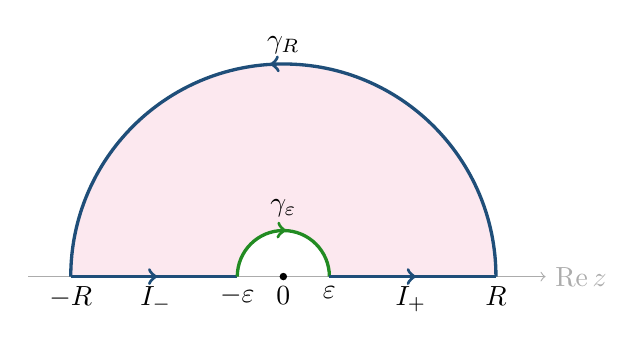
\begin{tikzpicture}[scale=0.9,
 decoration={markings,mark=at position 0.52 with {\arrow{>}}}]
 \fill[lightpink] (-3,0) arc[start angle=180,end angle=0,radius=3]
 --(0.65,0) arc[start angle=0,end angle=180,radius=0.65]--cycle;
 \draw[gray!65,->] (-3.6,0)--(3.7,0) node[right]{$\Real z$};
 \draw[very thick,courseblue,postaction={decorate}] (-3,0)--(-0.65,0);
 \draw[very thick,ForestGreen,postaction={decorate}] (-0.65,0)
 arc[start angle=180,end angle=0,radius=0.65];
 \draw[very thick,courseblue,postaction={decorate}] (0.65,0)--(3,0);
 \draw[very thick,courseblue,postaction={decorate}] (3,0)
 arc[start angle=0,end angle=180,radius=3];
 \node[below] at (-3,0){$-R$};\node[below] at (3,0){$R$};
 \node[below] at (-0.65,0){$-\varepsilon$};
 \node[below] at (0.65,0){$\varepsilon$};
 \fill (0,0) circle(1.5pt) node[below]{$0$};
 \node[above] at (0,3){$\gamma_R$};
 \node[above] at (0,0.7){$\gamma_\varepsilon$};
 \node[below] at (-1.8,0){$I_-$};\node[below] at (1.8,0){$I_+$};
\end{tikzpicture}
\end{center}
For this contour we have
\begin{equation}\label{eq:indented}
 \int_{I_-}f+\int_{\gamma_\varepsilon}f+
 \int_{I_+}f+\int_{\gamma_R}f=0.
\end{equation}
Here is a direct justification using facts already proved, without
assuming a general version of Cauchy's theorem for arbitrary regions.
The exponential series gives
\begin{equation}\label{eq:split}
 f(z)=-\frac{i}{z}+E(z),\qquad
 E(z)=-\sum_{n=2}^{\infty}\frac{i^n z^{n-2}}{n!}
 =\frac12+\frac{iz}{6}-\frac{z^2}{24}+\cdots.
\end{equation}
The series for $E$ converges everywhere, so $E$ is entire and
$\int_\Gamma E=0$. Also,
\[
 \int_{I_-}\frac{dz}{z}+\int_{I_+}\frac{dz}{z}
 =\log\frac{\varepsilon}{R}+\log\frac{R}{\varepsilon}=0,
\]
while the two semicircles contribute
\[
 \int_{\gamma_\varepsilon}\frac{dz}{z}=\int_\pi^0 i\,d\theta=-i\pi,
 \qquad
 \int_{\gamma_R}\frac{dz}{z}=\int_0^\pi i\,d\theta=i\pi.
\]
Thus $\int_\Gamma dz/z=0$, and \eqref{eq:split} proves
\eqref{eq:indented}.


\subsection{Estimating the arcs and taking limits}
\textbf{The large semicircle.} In the upper half-plane,
$|e^{iz}|=e^{-\Imag z}\leq1$, so $|1-e^{iz}|\leq2$.
On $\gamma_R$, therefore, $|f(z)|\leq2/R^2$. The ML estimate gives
\begin{equation}\label{eq:large-arc}
 \left|\int_{\gamma_R}f\right|
 \leq\frac{2}{R^2}\,\pi R=\frac{2\pi}{R}\longrightarrow0
 \qquad(R\to\infty).
\end{equation}

\textbf{The small semicircle.} Use \eqref{eq:split}. Since
$\gamma_\varepsilon$ goes clockwise, its angle decreases from $\pi$ to $0$:
\begin{align*}
 \int_{\gamma_\varepsilon}f(z)\,dz
 &=\int_\pi^0\frac{-i}{\varepsilon e^{i\theta}}
       i\varepsilon e^{i\theta}\,d\theta
       +\int_{\gamma_\varepsilon}E(z)\,dz\\
 &=-\pi+\int_{\gamma_\varepsilon}E(z)\,dz.
\end{align*}
As $E$ is continuous near $0$, there is a constant $M$ such that
$|E(z)|\leq M$ for $|z|\leq1$. For $0<\varepsilon\leq1$,
\[
 \left|\int_{\gamma_\varepsilon}E(z)\,dz\right|
 \leq M\pi\varepsilon\longrightarrow0.
\]
Consequently,
\begin{equation}\label{eq:small-arc}
 \lim_{\varepsilon\to0^+}\int_{\gamma_\varepsilon}f=-\pi.
\end{equation}

\textbf{The real intervals.} Their sum is
\begin{align*}
 \int_{I_-}f+\int_{I_+}f
 &=\int_{-R}^{-\varepsilon}\frac{1-e^{ix}}{x^2}\,dx
   +\int_\varepsilon^R\frac{1-e^{ix}}{x^2}\,dx\\
 &=2\int_\varepsilon^R\frac{1-\cos x}{x^2}\,dx.
\end{align*}
The imaginary parts cancel because $\sin x/x^2$ is odd. Substitution
into \eqref{eq:indented} yields
\[
 2\int_\varepsilon^R\frac{1-\cos x}{x^2}\,dx
 =-\int_{\gamma_\varepsilon}f-\int_{\gamma_R}f.
\]
First let $R\to\infty$ using \eqref{eq:large-arc}, and then let
$\varepsilon\to0^+$ using \eqref{eq:small-arc}. We obtain
\[
 2\int_0^\infty\frac{1-\cos x}{x^2}\,dx=\pi,
\]
which proves \eqref{eq:cosine-goal}.

\begin{remark}[The complex integral at the origin]
The symmetric limit
\[
 \lim_{\varepsilon\to0^+}\left(
 \int_{-\infty}^{-\varepsilon}\frac{1-e^{ix}}{x^2}\,dx+
 \int_\varepsilon^\infty\frac{1-e^{ix}}{x^2}\,dx\right)=\pi
\]
is a \emph{Cauchy principal value}. The separate one-sided complex
integrals do not converge at $0$, because $f(x)=-i/x+O(1)$.
The real part, however, has an ordinary convergent improper integral,
with value $\pi$ on $\R$ and $\pi/2$ on $(0,\infty)$.
\end{remark}

\end{document}
